    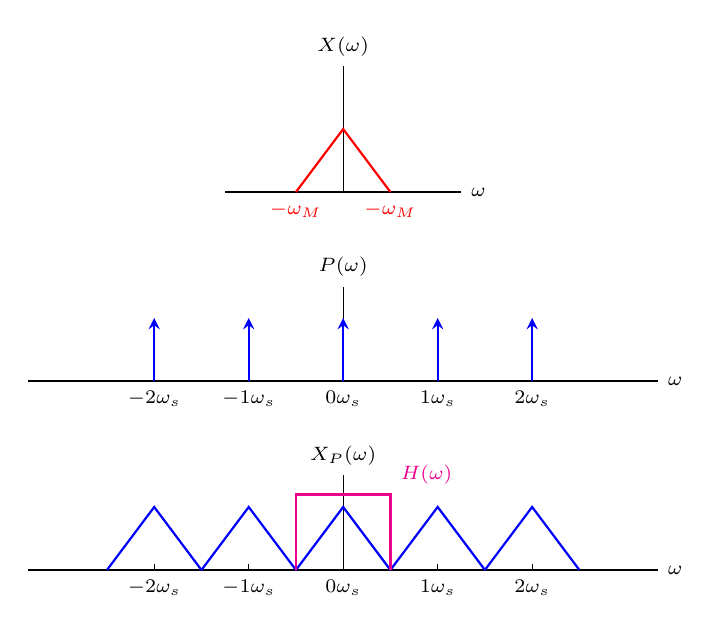
\begin{tikzpicture}[xscale=0.5, yscale=0.8]
    	\def\wm{1.2}
    	\def\ws{2.4}    	
        \draw (0,0) ++(-3,0) -- ++(6,0) node[anchor=west] {\scriptsize $\omega$};
        \draw (0,0) -- ++(0,2) node[anchor=south] {\scriptsize$X(\omega)$};
        \draw[red, thick] (0,0) ++(-\wm,0) node[anchor=north] {\scriptsize$-\omega_M$} -- ++(\wm,1) -- +(\wm, -1) node[anchor=north] {\scriptsize$-\omega_M$};

        \begin{scope}[yshift=-3cm]
	        \draw (0,0) ++(-8,0) -- ++(16,0) node[anchor=west] {\scriptsize $\omega$};
	        \draw (0,0) -- ++(0,1.5) node[anchor=south] {\scriptsize$P(\omega)$};
	        \foreach \w in {-2, -1, 0, 1, 2}
	        {
	            \draw[blue, thick, -stealth] (\w*\ws, 0) node[anchor=north, color=black] {\scriptsize $\w\omega_s$} -- ++(0, 1);
	        }
	\end{scope}
	
        \begin{scope}[yshift=-6cm]
	        \draw (0,0) ++(-8,0) -- ++(16,0) node[anchor=west] {\scriptsize $\omega$};
	        \draw (0,0) -- ++(0,1.5) node[anchor=south] {\scriptsize$X_P(\omega)$};
		\def\tantheta{1/\wm}	
	        \foreach \w in {-2, -1, 0, 1, 2}
	        {
	
	            \draw[red, red] (\w*\ws, 0) ++(-\wm, 0) -- ++(\wm, 1) -- ++(\wm, -1);
	            \node at  (\w*\ws, 0) [anchor=north, color=black] {\scriptsize $\w\omega_s$};
	            \draw (\w*\ws, 0)  -- ++(0, 0.1);

	            \draw [blue, thick]  (\w*\ws - \wm, {(2*\wm - \ws)*\tantheta})  -- ++({(2*\wm - \ws)}, 0) -- ++({\ws - \wm)},{(\ws - \wm)*\tantheta}) -- ++({\ws - \wm)},{-(\ws - \wm)*\tantheta});
	
	        }
	            \draw [blue, thick]  (3*\ws - \wm, {(2*\wm - \ws)*\tantheta})  -- ++({(2*\wm - \ws)}, 0);
\pause
	            \draw[thick, magenta] (-\ws/2, 0) |- (\ws/2, 1.2) node [anchor=south west] {\scriptsize $H(\omega)$} -- ++(0, -1.2);
			
		\end{scope}	

    \end{tikzpicture} 